\chapter{Partial Results}

\label{ch: Res}

The expected result of this work is a software capable of correctly estimating the parameters of Type-3 WTG's mathematical model. To do so, the software will apply the proposed estimation method comprises of MVMO and TSM methods combined. 

The measurements will be obtained from a small power system simulated on specific software, such as DIgSILENT or MATLAB. At first, the model proposed in \cite{Erlich2012} will be employed, but it can be further changed if needed. Also, other estimation methods, such as Particle Swarm Optimization, Differential Evolution or Kalman Filters, may be implemented for comparison purposes.

The hybrid approach for parameters estimation presented in this work is already implemented and have shown great results for different models. The approach was used to estimate parameters of simpler systems, such as the spring-mass system, as depicted on Figure \ref{fig: spring-mass}. 

\begin{figure}[h]
	\caption{Results of method for spring-mass system}
	\begin{center}
		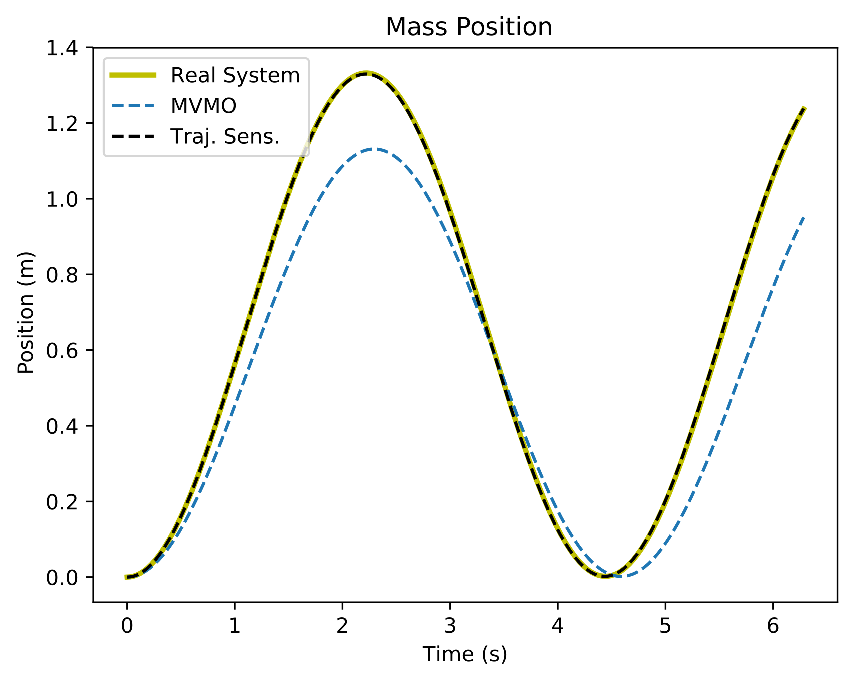
\includegraphics[scale=0.8]{Images/SpringMass.eps}
	\end{center}
	\label{fig: spring-mass}
\end{figure}

When compared to the methods alone, the hybrid approach provides a result faster than MVMO but slower than TSM, as shown in Table \ref{tab: SM}. The tolerance for all three approaches was set at $0.5 \times 10^{-3}$ and the final error obtained for all simulations was adequate.

\begin{table}[]
	\caption{Comparison of approaches}
	\begin{center}
	\begin{tabular}{c|c|c}
		Approach & Time & Error \\
		\hline
		TSM  & $7 \ s$  & $4.2\times 10^{-7}$ \\
		MVMO  & $136 \ min$  & $5.0\times 10^{-4}$\\
		Hybrid  & $24 \ min$  & $1.9\times 10^{-7}$
	\end{tabular}
	\end{center}
	\label{tab: SM}
\end{table}

However, the convergence region of TSM is extremely limited, diverging from initial points far enough from the real values. The convergence region when the real values are $k = 6.0 \ N/m$ and $m = 3.0 \ kg$ was obtained in \cite{Ecyo} and is shown in Figure \ref{fig: conv_reg}. For comparison, the MVMO and the hybrid approach converge for the entire search region displayed on the graph.

\begin{figure}[h]
	\caption{Convergence region of Trajectory Sensitivity Method}
	\begin{center}
		\includegraphics[scale=0.8]{Images/Conv_reg.eps}
	\end{center}
	\label{fig: conv_reg}
	\legend{Source: Adapted from \cite{Ecyo}}
\end{figure}

This application was also employed on parameter estimation of Z-IM load model and is subject of a paper presented by the author on the 2019 Canadian Conference on Electrical and Computer Engineering. The result of the parameter estimation for the Z-IM Load Model presented on the conference is displayed on Figure \ref{fig: ZIM}.

\begin{figure}[h]
	\caption{Result of parameter estimation for Z-IM Load Model}
	\begin{center}
		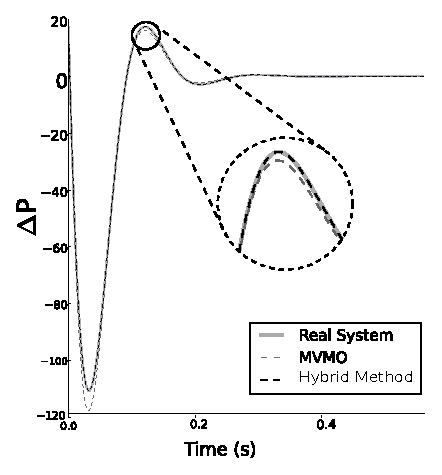
\includegraphics[scale=1]{Images/ZIM.eps}
	\end{center}
	\label{fig: ZIM}
	\legend{Source: \cite{Gomes2019}}
\end{figure}

\section{Ongoing Progress}

With the methods already implemented and tested, the focus is now on the DFIG model. The model has presented some results, but it is not as accurate as expected, requiring some studies about this topic. Also, the GUI is under development and already has some features implemented using Python's library \textit{Tkinter}. A proposal to also develop features using \textit{Qt}, a different GUI tool package, is currently under consideration.